\PassOptionsToPackage{unicode=true}{hyperref} % options for packages loaded elsewhere
\PassOptionsToPackage{hyphens}{url}
\PassOptionsToPackage{dvipsnames,svgnames*,x11names*}{xcolor}
%
\documentclass[]{article}
\usepackage{lmodern}
\usepackage{amssymb,amsmath}
\usepackage{ifxetex,ifluatex}
\usepackage{fixltx2e} % provides \textsubscript
\ifnum 0\ifxetex 1\fi\ifluatex 1\fi=0 % if pdftex
  \usepackage[T1]{fontenc}
  \usepackage[utf8]{inputenc}
  \usepackage{textcomp} % provides euro and other symbols
\else % if luatex or xelatex
  \usepackage{unicode-math}
  \defaultfontfeatures{Ligatures=TeX,Scale=MatchLowercase}
\fi
% use upquote if available, for straight quotes in verbatim environments
\IfFileExists{upquote.sty}{\usepackage{upquote}}{}
% use microtype if available
\IfFileExists{microtype.sty}{%
\usepackage[]{microtype}
\UseMicrotypeSet[protrusion]{basicmath} % disable protrusion for tt fonts
}{}
\IfFileExists{parskip.sty}{%
\usepackage{parskip}
}{% else
\setlength{\parindent}{0pt}
\setlength{\parskip}{6pt plus 2pt minus 1pt}
}
\usepackage{xcolor}
\usepackage{hyperref}
\hypersetup{
            colorlinks=true,
            linkcolor=blue,
            citecolor=Blue,
            urlcolor=Blue,
            breaklinks=true}
\urlstyle{same}  % don't use monospace font for urls
\usepackage{longtable,booktabs}
% Fix footnotes in tables (requires footnote package)
\IfFileExists{footnote.sty}{\usepackage{footnote}\makesavenoteenv{longtable}}{}
\usepackage{graphicx,grffile}
\makeatletter
\def\maxwidth{\ifdim\Gin@nat@width>\linewidth\linewidth\else\Gin@nat@width\fi}
\def\maxheight{\ifdim\Gin@nat@height>\textheight\textheight\else\Gin@nat@height\fi}
\makeatother
% Scale images if necessary, so that they will not overflow the page
% margins by default, and it is still possible to overwrite the defaults
% using explicit options in \includegraphics[width, height, ...]{}
\setkeys{Gin}{width=\maxwidth,height=\maxheight,keepaspectratio}
\setlength{\emergencystretch}{3em}  % prevent overfull lines
\providecommand{\tightlist}{%
  \setlength{\itemsep}{0pt}\setlength{\parskip}{0pt}}
\setcounter{secnumdepth}{5}
% Redefines (sub)paragraphs to behave more like sections
\ifx\paragraph\undefined\else
\let\oldparagraph\paragraph
\renewcommand{\paragraph}[1]{\oldparagraph{#1}\mbox{}}
\fi
\ifx\subparagraph\undefined\else
\let\oldsubparagraph\subparagraph
\renewcommand{\subparagraph}[1]{\oldsubparagraph{#1}\mbox{}}
\fi

% set default figure placement to htbp
\makeatletter
\def\fps@figure{htbp}
\makeatother


%% pandoc-secnos: required package
\usepackage{cleveref}

%% pandoc-eqnos: disable brackets around cleveref numbers
\creflabelformat{equation}{#2#1#3}

\date{}

\begin{document}

\newcommand{\df}[1]{\frac{\partial}{\partial #1}}

\hypertarget{principal-component-analysis}{%
\section{Principal Component
Analysis}\label{principal-component-analysis}}

\hypertarget{introduction}{%
\subsection{Introduction}\label{introduction}}

Suppose that, as usual, we begin with a collection of measurements of
different features for a group of samples. Some of these measurements
will tell us quite a bit about the difference among our samples, while
others may contain relatively little information. For example, if we are
analyzing the effect of a certain weight loss regimen on a group of
people, the age and weight of the subjects may have a great deal of
influence on how successful the regimen is, while their blood pressure
might not. One way to help identify which features are more significant
is to ask whether or not the feature varies a lot among the different
samples. If nearly all the measurements of a feature are the same, it
can't have much power in distinguishing the samples, while if the
measurements vary a great deal then that feature has a chance to contain
useful information.

In this section we will discuss a way to measure the variability of
measurements and then introduce principal component analysis (PCA). PCA
is a method for finding which linear combinations of measurements have
the greatest variability and therefore might contain the most
information. It also allows us to identify combinations of measurements
that don't vary much at all. Combining this information, we can
sometimes replace our original system of features with a smaller set
that still captures most of the interesting information in our data, and
thereby find hidden characteristics of the data and simplify our
analysis a great deal.

\hypertarget{variance-and-covariance}{%
\subsection{Variance and Covariance}\label{variance-and-covariance}}

\hypertarget{variance}{%
\subsubsection{Variance}\label{variance}}

Suppose that we have a collection of measurements \((x_1,\ldots, x_n)\)
of a particular feature \(X\). For example, \(x_i\) might be the initial
weight of the \(ith\) participant in our weight loss study. The mean of
the values \((x_1,\ldots, x_n)\) is

\[
\mu_{X} = \frac{1}{n}\sum_{i=1}^{n} x_{i}.
\]

The simplest measure of the variability of the data is called its
\emph{variance.}

\textbf{Definition:} The (sample) variance of the data
\(x_1,\ldots, x_n\) is

\begin{equation}
\sigma_{X}^2 = \frac{1}{n}\sum_{i=1}^{n} (x_{i}-\mu_{X})^2 = \frac{1}{n}\sum_{i=1}^{n} x_{i}^2 - \mu_{X}^2
\label{eq:variance}\end{equation}

The square root of the variance is called the \emph{standard deviation.}

As we see from the formula, the variance is a measure of how `spread
out' the data is from the mean.

Recall that in our discussion of linear regression we thought of our set
of measurements \(x_1,\ldots, x_n\) as a vector -- it's one of the
columns of our data matrix. From that point of view, the variance has a
geometric interpretation -- it is \(\frac{1}{N}\) times the square of
the distance from the point \(X=(x_1,\ldots, x_n)\) to the point
\(\mu_{X}(1,1,\ldots,1)=\mu_{X}E\):

\begin{equation}
\sigma_{X}^2 = \frac{1}{n}(X-\mu_{X}E)\cdot(X-\mu_{X}E)  = \frac{1}{n}\|X-\mu_{X}E\|^2.
\label{eq:variancedot}\end{equation}

\hypertarget{covariance}{%
\subsubsection{Covariance}\label{covariance}}

The variance measures the dispersion of measures of a single feature.
Often, we have measurements of multiple features and we might want to
know something about how two features are related. The \emph{covariance}
is a measure of whether two features tend to be related, in the sense
that when one increases, the other one increases; or when one increases,
the other one decreases.

\textbf{Definition:} Given measurements \((x_1,\ldots, x_n)\) and
\((y_1,\ldots, y_n)\) of two features \(X\) and \(Y\), the covariance of
\(X\) and \(Y\) is

\begin{equation}
\sigma_{XY} = \frac{1}{N}\sum_{i=1}^{N} x_iy_i
\label{eq:covariancedot}\end{equation}

There is a nice geometric interpretation of this, as well, in terms of
the dot product. If \(X=(x_1,\ldots, x_n)\) and \(Y=(y_1\ldots,y_n)\)
then

\[
\sigma_{XY} = \frac{1}{N} ((X-\mu_{X})\cdot (Y-\mu_{Y})).
\]

From this point of view, we can see that \(\sigma_{XY}\) is positive if
the \(X-\mu_{X}\) and \(Y-\mu_{Y}\) vectors ``point roughly in the same
direction'' and its negative if they ``point roughly in the opposite
direction.''

\hypertarget{correlation}{%
\subsubsection{Correlation}\label{correlation}}

One problem with interpreting the variance and covariance is that we
don't have a scale -- for example, if \(\sigma_{XY}\) is large and
positive, then we'd like to say that \(X\) and \(Y\) are closely
related, but it could be just that the entries of \(X-\mu_{X}\) and
\(Y-\mu_{Y}\) are large. Here, though, we can really take advantage of
the geometric interpretation. Recall that the dot product of two vectors
satisfies the formula

\[
a \cdot b = \|a\|\|b\|\cos(\theta)
\]

where \(\theta\) is the angle between \(a\) and \(b\). So

\[
\cos(\theta) = \frac{a\cdot b}{\|a\|\|b\|}.
\]

Let's apply this to the variance and covariance, by noticing that

\[
\frac{(X-\mu_{X})\cdot (Y-\mu_{Y})}{\|(X-\mu_{X})\|\|(Y-\mu_{Y})\|} = \frac{\sigma_{XY}}{\sigma_{XX}\sigma_{YY}}
\]

so the quantity

\begin{equation}
r_{XY} = \frac{\sigma_{XY}}{\sigma_{X}\sigma_{Y}}
\label{eq:rxy}\end{equation}

measures the cosine of the angle between the vectors \(X-\mu_{X}\)A and
\(Y-\mu_{Y}\).

\textbf{Definition:} The quantity \(r_{XY}\) defined in \cref{eq:rxy} is
called the (sample) \emph{correlation coefficient} between \(X\) and
\(Y\). We have \(0\le |r_{XY}|\le 1\) with \(r_{XY}=\pm 1\) if and only
if the two vectors \(X-\mu_{X}\) and \(Y-\mu_{Y}\) are collinear in
\(\mathbf{R}^{n}\).

\Cref{fig:corrfig} illustrates data with different values of the
correlation coefficient.

\begin{figure}
\hypertarget{fig:corrfig}{%
\centering
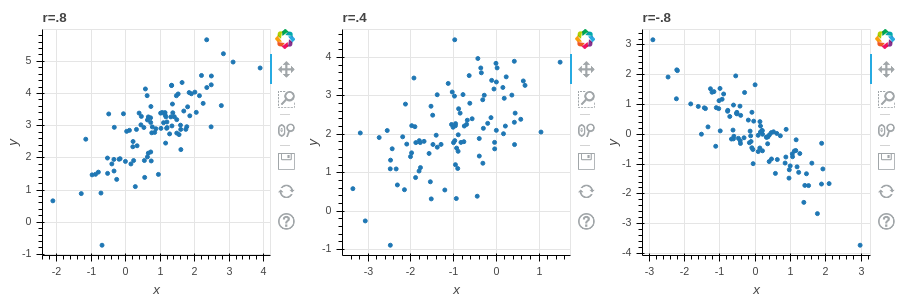
\includegraphics[width=0.5\textwidth,height=\textheight]{../img/correlation.png}
\caption{Correlation}\label{fig:corrfig}
}
\end{figure}

\hypertarget{sec:covarmat}{%
\subsubsection{The covariance matrix}\label{sec:covarmat}}

In a typical situation we have many features for each of our (many)
samples, that we organize into a data matrix \(X\). To recall, each
column of \(X\) corresponds to a feature that we measure, and each row
corresponds to a sample. For example, each row of our matrix might
correspond to a person enrolled in a study, and the columns correspond
to height (cm), weight (kg), systolic blood pressure, and age (in
years):

\begin{longtable}[]{@{}lrrrr@{}}
\caption{A sample data matrix \(X\) \label{tbl:data}}\tabularnewline
\toprule
sample & Ht & Wgt & Bp & Age\tabularnewline
\midrule
\endfirsthead
\toprule
sample & Ht & Wgt & Bp & Age\tabularnewline
\midrule
\endhead
A & 180 & 75 & 110 & 35\tabularnewline
B & 193 & 80 & 130 & 40\tabularnewline
\ldots{} & \ldots{} & \ldots{} & \ldots{} & \ldots{}\tabularnewline
U & 150 & 92 & 105 & 55\tabularnewline
\bottomrule
\end{longtable}

If we have multiple features, as in this example, we might be interested
in the variance of each feature and all of their mutual covariances.
This ``package'' of information can be obtained ``all at once'' by
taking advantage of some matrix algebra.

\textbf{Definition:} Let \(X\) be a \(k\times N\) data matrix, where the
\(N\) columns of \(X\) correspond to different features and the \(k\)
rows to different samples. Let \(X_{0}\) be the centered version of this
data matrix, obtained by subtracting the mean \(\mu_{i}\) of column
\(i\) from all the entries \(x_{si}\) in that column. Then the
\(N\times N\) symmetric matrix

\[
D_{0} = \frac{1}{N}X_{0}^{\intercal}X_{0}
\]

is called the (sample) covariance matrix for the data.

\textbf{Proposition:} The diagonal entries \(d_{ii}\) of \(D_{0}\) are
the variances of the columns of \(X\):

\[
d_{ii} = \sigma_{i}^2 = \frac{1}{N}\sum_{s=1}^{k}(x_{si}-\mu_i)^2
\]

and the off-diagonal entries \(d_{ij} = d_{ji}\) are the covariances of
the \(i^{th}\) and \(j^{th}\) columns of \(X\):

\[
d_{ij} = \sigma_{ij} = \frac{1}{N}\sum_{s=1}^{k}(x_{si}-\mu_{i})(x_{sj}-\mu_{j})
\]

\textbf{Proof:} This follows from the definitions, but it's worth
checking the details, which we leave as an exercise.

\hypertarget{linear-combinations-of-features-scores}{%
\subsubsection{Linear Combinations of Features
(Scores)}\label{linear-combinations-of-features-scores}}

Sometimes useful information about our data can be revealed if we
combine different measurements together to obtain a ``hybrid'' measure
that captures something interesting. For example, in the Auto MPG
dataset that we studied in the section on Linear Regression, we looked
at the influence of both vehicle weight \(w\) and engine displacement
\(e\) on gas mileage; perhaps their is some value in considering a
hybrid ``score'' defined as \[
S = a*w + b*e
\] for some constants \(a\) and \(b\) -- maybe by choosing a good
combination we could find a better predictor of gas mileage than using
one or the other of the features individually.

As another example, suppose we are interested in the impact of the
nutritional content of food on weight gain in a study. We know that both
calorie content and the level dietary fiber contribute to the weight
gain of participants eating this particular food; maybe there is some
kind of combined ``calorie/fiber'' score we could introduce that
captures the impact of that food better.

\textbf{Definition:} Let \(X_{0}\) be a (centered) \(k\times N\) data
matrix giving information about \(N\) features for each of \(k\)
samples. A linear synthetic feature, or a linear score, is a linear
combination of the \(N\) features. The linear score is defined by
constants \(a_{1},\ldots, a_{n}\) so that If \(y_{1},\ldots, y_{N}\) are
the values of the features for a particular sample, then the linear
score for that sample is

\[
S = a_{1}y_{1}+a_{2}y_{2}+\cdots+a_{N}y_{N}
\]

\textbf{Lemma:} The values of the linear score for each of the \(k\)
samples can be calculated as

\begin{equation}
\left[\begin{matrix} S_{1} \\ \vdots \\ S_{k}\\ \end{matrix}\right] =
X_{0}\left[
\begin{matrix} a_{1} \\ \vdots \\ a_{N}\end{matrix}\right].
\label{eq:linearscore}\end{equation}

\textbf{Proof:} Multiplying a matrix by a column vector computes a
linear combination of the columns -- that's what this lemma says.
Exercise 3 asks you to write out the indices and make sure you believe
this.

\hypertarget{mean-and-variance-of-scores}{%
\subsubsection{Mean and variance of
scores}\label{mean-and-variance-of-scores}}

When we combine features to make a hybrid score, we assume that the
features were centered to begin with, so that each features has mean
zero. As a result, the mean of the hybrid features is again zero.

\textbf{Lemma:} A linear combination of features with mean zero again
has mean zero.

\textbf{Proof:} Let \(S_{i}\) be the score for the \(i^{th}\) sample, so
\[
S_{i} = \sum_{j=1}^{N} x_{ij}a_{j}.
\] where \(X_{0}\) has entries \(x_{ij}\). Then the mean value of the
score is \[
\mu_{S} = \frac{1}{k}\sum_{i=1}^{k} S_{i} = \frac{1}{k}\sum_{i=1}^{k}\sum_{j=1}^{N} x_{ij}a_{j}.
\] Reversing the order of the sum yields \[
\mu_{S} = \frac{1}{k}\sum_{j=1}^{N}\sum_{i=1}^{k} x_{ij}a_{j} = \sum_{j=1}^{N} a_{j}\frac{1}{k}(\sum_{i=1}^{k} x_{ij})=
\sum_{j=1}^{N}a_{j}\mu_{j}=0
\] where \(\mu_{j}=0\) is the mean of the \(j^{th}\) feature (column) of
\(X_{0}\).

The variance is more interesting, and gives us an opportunity to put the
covariance matrix to work. Remember from \ref{eq:variancedot} that,
since a score \(S\) has mean zero, it's variance is
\(\sigma_{S}^2=S\cdot S\) -- where here the score \(S\) is represented
by the column vector with entries \(S_{1},\ldots S_{k}\) as in
\cref{eq:linearscore}.

\textbf{Lemma:} The variance of the score \(S\) with weights
\(a_1,\ldots a_N\) is \begin{equation}
\sigma_{S}^2 = a^{\intercal}D_{0}a = \left[\begin{matrix}a_{1} & \cdots & a_{N}\end{matrix}\right]D_{0}
\left[\begin{matrix} a_{1} \\ \vdots \\ a_{N}\end{matrix}\right]
\label{eq:ada}\end{equation} More generally, if \(S_{1}\) and \(S_{2}\)
are scores with weights \(a_1,\ldots, a_N\) and \(b_1,\ldots, b_N\)
respectively, then the covariance \(\sigma_{S_{1}S_{2}}\) is \[
\sigma_{S_{1}S_{2}} = a^{\intercal}D_{0}b.
\]

\textbf{Proof:} From \cref{eq:variancedot} and \ref{eq:linearscore} we
know that \[
\sigma_{S}^2 = S\cdot S
\] and \[
S = X_{0}a.
\] Since \(S\cdot S = \frac{1}{N}S^{\intercal}S\), this gives us \[
\sigma_{S}^2 = \frac{1}{N}(X_{0}a)^{\intercal}(X_{0}a) = \frac{1}{N}a^{\intercal}X_{0}^{\intercal}X_{0}a = a^{\intercal}D_{0}a
\] as claimed.

For the covariance, use a similar argument with \cref{eq:covariancedot}
and \cref{eq:linearscore}. writing
\(\sigma_{S_{1}S_{2}}=\frac{1}{N}S_{1}\cdot S_{2}\) and the fact that
\(S_{1}\) and \(S_{2}\) can be written as \(X_{0}a\) and \(X_{0}b\).

The point of this lemma is that the covariance matrix contains not just
the variances and covariances of the original features, but also enough
information to construct the variances and covariances for \emph{any
linear combination of features.}

In the next section we will see how to exploit this idea to reveal
hidden structure in our data.

\hypertarget{geometry-of-scores}{%
\subsubsection{Geometry of Scores}\label{geometry-of-scores}}

Let's begin by looking at \cref{fig:pcasimfig}, which shows a scatter
plot of some simulated data having \(50\) samples and two features. This
data has been centered, so it can be represented in a \(50\times 2\)
data matrix \(X_{0}\) each row of which is the coordinates \((x_0,x_1)\)
of one of the points in the picture.

The scatter plot shows that the data points are arranged in a more or
less elliptical cloud oriented at an angle to the \(xy\)-axes which
represent the two given features. The two individual histograms show the
distribution of the two features -- each has mean zero, with the
\(x\)-features distributed between \(-2\) and \(2\) and the \(y\)
feature between \(-4\) and \(4\). Looking just at the two features
individually, meaning only at the two histograms, we can't see the
overall elliptical structure.

\begin{figure}
\hypertarget{fig:pcasimfig}{%
\centering
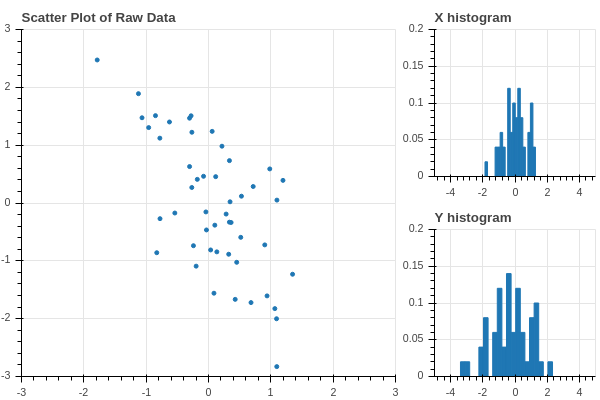
\includegraphics[width=0.5\textwidth,height=\textheight]{../img/PCAsimulated-1.png}
\caption{Simulated Data with Two Features}\label{fig:pcasimfig}
}
\end{figure}

How can we get a better grip on our data in this situation? We can try
to find a ``direction'' in our data that better illuminates the
variation of the data. For example, suppose that we pick a unit vector
at the origin pointing in a particular direction in our data. See
\cref{fig:pcasimfig-1}.

\begin{figure}
\hypertarget{fig:pcasimfig-1}{%
\centering
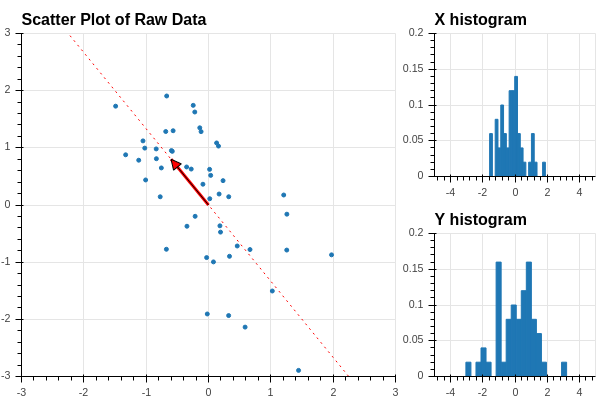
\includegraphics[width=0.5\textwidth,height=\textheight]{../img/PCAsimulated-2.png}
\caption{A direction in the data}\label{fig:pcasimfig-1}
}
\end{figure}

Now we can orthogonally project the datapoints onto the line defined by
this vector, as shown in \cref{fig:pcasimfig-2}.

\begin{figure}
\hypertarget{fig:pcasimfig-2}{%
\centering
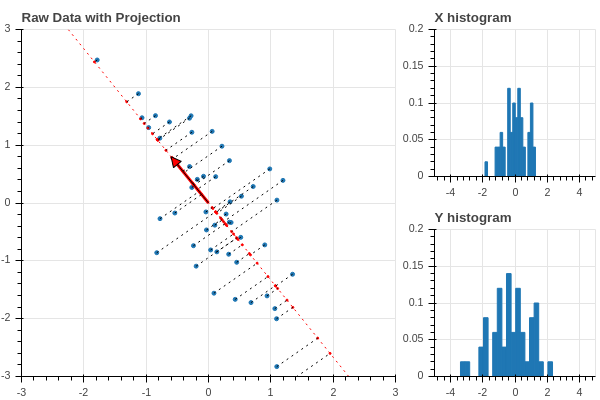
\includegraphics[width=0.5\textwidth,height=\textheight]{../img/PCAsimulated-3.png}
\caption{Projecting the datapoints}\label{fig:pcasimfig-2}
}
\end{figure}

Recall that if the unit vector is defined by coordinates
\(u=[u_0,u_1]\), then the orthogonal projection of the point \(x\) with
coordinates \((x_0,x_1)\) is \((x\cdot u)u\). Now \[
x\cdot u = u_0 x_0 + u_1 x_1
\] so the coordinates of the points along the line defined by \(u\) are
the values of the score \(Z\) defined by \(u=[u_0,u_1]\). Using our work
in the previous section, we see that we can find all of these
coordinates by matrix multiplication: \[
Z = X_0 u
\] where \(X_0\) is our data matrix. Now let's add a histogram of the
values of \(Z\) to our picture:

\begin{figure}
\hypertarget{fig:pcasimfig-3}{%
\centering
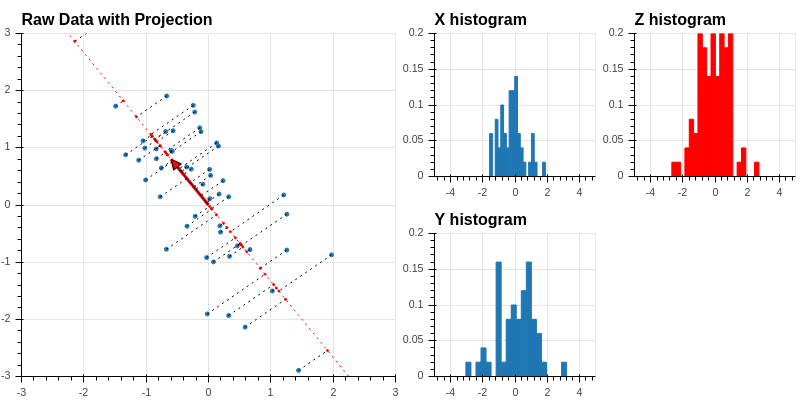
\includegraphics[width=0.5\textwidth,height=\textheight]{../img/PCAsimulated-4.png}
\caption{Distribution of Z}\label{fig:pcasimfig-3}
}
\end{figure}

This histogram shows the distribution of the values of \(Z\) along the
tilted line defined by the unit vector \(u\).

Finally, using our work on the covariance matrix, we see that the
variance of \(Z\) is given by \[
\sigma_{Z}^2 = \frac{1}{50}u^{\intercal}X_{0}^{\intercal}X_{0}u = u^{\intercal}D_{0}u
\] where \(D_{0}\) is the covariance matrix of the data \(X_{0}\).

\textbf{Lemma:} Let \(X_{0}\) be a \(k\times N\) centered data matrix,
and let \(D_{0}=\frac{1}{N}X_{0}^{\intercal}X_{0}\) be the associated
covariance matrix. Let \(u\) be a unit vector in ``feature space''
\(\mathbf{R}^{N}\). Then the score \(S=X_{0}u\) can be interpreted as
the coordinates of the points of \(X_{0}\) projected onto the line
generated by \(u\). The variance \[
\sigma^{2}_{S} = u^{\intercal}D_{0}u = \sum_{i=1}^{k} s_{i}^2
\] where \(s_{i} = X_{0}[i,:]u\) is the dot product of the \(i^{th}\)
row \(X_{0}[i,:]\) with \(u\). It measures the variability in the data
``in the direction of the unit vector \(u\)''.

\hypertarget{principal-components}{%
\subsubsection{Principal Components}\label{principal-components}}

\hypertarget{change-of-variance-with-direction}{%
\paragraph{Change of variance with
direction}\label{change-of-variance-with-direction}}

As we've seen in the previous section, if we choose a unit vector \(u\)
in the feature space and find the projection \(X_{0}u\) of our data onto
the line through \(u\), we get a ``score'' that we can use to measure
the variance of the data in the direction of \(u\). What happens as we
vary \(u\)?

To study this question, let's continue with our simulated data from the
previous section, and introduce a unit vector \[
u(\theta) = \left[\begin{matrix} \cos(\theta) & \sin(\theta)\end{matrix}\right].
\] This is in fact a unit vector, since
\(\sin^2(\theta)+\cos^2(\theta)=1\), and it is oriented at an angle
\(\theta\) from the \(x\)-axis.

The variance of the data in the direction of \(u(\theta)\) is given by
\[
\sigma_{\theta}^2 = u(\theta)^{\intercal}D_{0}u(\theta).
\]

A plot of this function for the data we have been considering is in
\cref{fig:pcatheta}. As you can see, the variance goes through two full
periods with the angle, and it reaches a maximum and minimum value at
intervals of \(\pi/2\) -- so the two angles where the variance are
maximum and minimum are orthogonal to one another.

\begin{figure}
\hypertarget{fig:pcatheta}{%
\centering
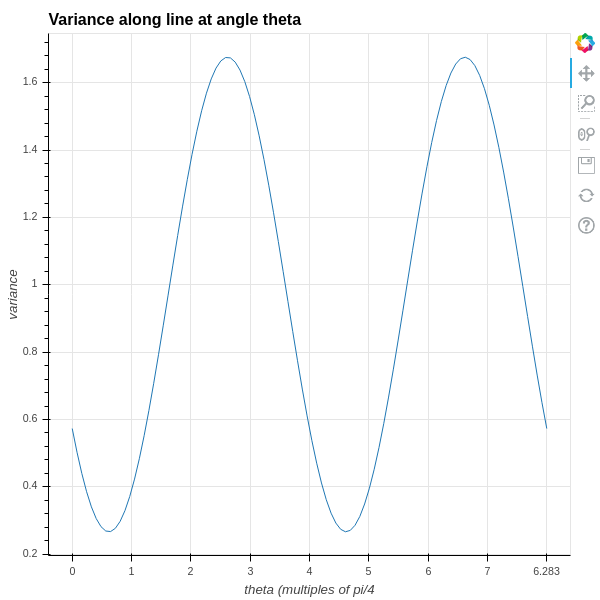
\includegraphics[width=0.25\textwidth,height=\textheight]{../img/PCAtheta.png}
\caption{Change of variance with angle theta}\label{fig:pcatheta}
}
\end{figure}

The two directions where the variance is maximum and minimum are drawn
on the original data scatter plot in \cref{fig:pcaprincipal} .

\begin{figure}
\hypertarget{fig:pcaprincipal}{%
\centering
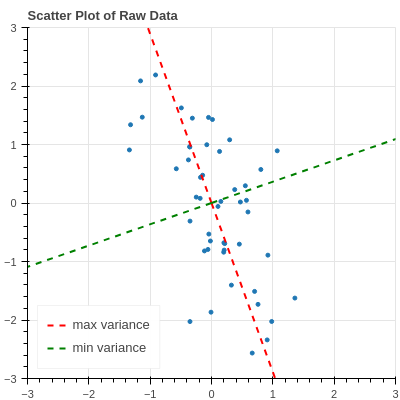
\includegraphics[width=0.25\textwidth,height=\textheight]{../img/PCAprincipal.png}
\caption{Data with principal directions}\label{fig:pcaprincipal}
}
\end{figure}

Let's try to understand why this is happening.

\hypertarget{directions-of-extremal-variance}{%
\paragraph{Directions of extremal
variance}\label{directions-of-extremal-variance}}

Given our centered, \(k\times N\) data matrix \(X_{0}\), with its
associated covariance matrix
\(D_{0}=\frac{1}{N}X_{0}^{\intercal}X_{0}\), we would like to find unit
vectors \(u\) in \(\mathbf{R}^{N}\) so that \[
\sigma_{u}^{2} = u^{\intercal}D_{0}u
\] reaches its maximum and its minimum. Here \(\sigma_{u}^2\) is the
variance of the ``linear score'' \(X_{0}u\) and it represents how
dispersed the data is in the ``u direction'' in \(\mathbf{R}^{N}\).

In this problem, remember that the coordinates of
\(u=(u_1,\ldots, u_{N})\) are the variables and the symmetric matrix
\(D_{0}\) is given. As usual, we to find the maximum and minimum values
of \(\sigma_{u}^{2}\), we should look at the partial derivatives of
\(\sigma_{u}^{2}\) with respect to the variables \(u_{i}\) and set them
to zero. Here, however, there is a catch -- we want to restrict \(u\) to
being a unit vector, with \(u\cdot u =\sum u_{i}^2=1\).

So this is a \emph{constrained optimization problem}:

\begin{itemize}
\tightlist
\item
  Find extreme values of the function \[
  \sigma_{u}^{2} = u^{\intercal}D_{0}u
  \]
\item
  Subject to the constraint \(\|u\|^2 = u\cdot u=1\) (or
  \(u\cdot u-1=0\))
\end{itemize}

As we learned in multivariate calculus, we can use the technique of
\emph{Lagrange Multipliers} to solve such a problem.

To apply this method, we introduce the function

\begin{equation}
S(u, \lambda) = u^{\intercal}D_{0}u - \lambda(u\cdot u -1)
\label{eq:lagrange}\end{equation}

Then we compute the gradient

\begin{equation}
\nabla S = \left[\begin{matrix} \frac{\partial S}{\partial u_{1}} \\ \vdots \\ \frac{\partial S}{\partial u_{N}} \\ \frac{\partial S}{\partial \lambda}\end{matrix}\right]
\label{eq:lagrangegradient}\end{equation}

and solve the system of equations \(\nabla S=0\). Here we have written
the gradient as a column vector for reasons that will become clearer
shortly.

Computing all of these partial derivatives looks messy, but actually if
we take advantage of matrix algebra it's not too bad. The following two
lemmas explain how to do this.

\textbf{Lemma}: Let \(M\) be a \(k\times N\) matrix with constant
coefficients and let \(u\) be a \(N\times 1\) column vector whose
entries are \(u_1,\ldots u_{N}\). The function \(F(u) = Mu\) is a linear
map from \(\mathbf{R}^{N}\to\mathbf{R}^{k}\). Its (total) derivative is
a linear map between the same vector spaces, and satisfies \[
D(F)(v) = Mv
\] for any \(N\times 1\) vector \(v\). If \(u\) is a \(1\times k\)
matrix, and \(G(u) = uM\), then \[
D(G)(v) = vM
\] for any \(1\times k\) vector \(v\). (This is the matrix version of
the derivative rule that \(\frac{d}{dx}(ax)=a\) for a constant \(a\).)

\textbf{Proof:} Since \(F:\mathbf{R}^{N}\to\mathbf{R}^{k}\), we can
write out \(F\) in more traditional function notation as \[
F(u) = (F_{1}(u_1,\ldots, u_N), \ldots, F_{k}(u_1,\ldots, u_{N})
\] where \[
F_{i}(u_1,\ldots u_N) = \sum_{j=1}^{N} m_{ij}u_{j}.
\] Thus \(\frac{\partial F_{i}}{\partial u_{j}} = m_{ij}\). The total
derivative \(D(F)\) is the linear map with matrix \[
D(F)_{ij} = \frac{\partial F_{i}}{\partial u_{j}} = m_{ij} = M.
\] The other result is proved the same way.

\textbf{Lemma}: Let \(D\) be a symmetric \(N\times N\) matrix with
constant entries and let \(u\) be an \(N\times 1\) column vector of
variables \(u_{1},\ldots, u_{N}\). Let \(F:\mathbf{R}^{N}\to R\) be the
function \(F(u) = u^{\intercal}Du\). Then the derivative gradient
\(\nabla_{u} F\) is a vector field -- that is, a vector-valued function
of \(u\), and is given by the formula \[
\nabla_{u} F = 2Du
\]

\textbf{Proof:} Let \(d_{ij}\) be the \(i,j\) entry of \(D\). We can
write out the function \(F\) to obtain \[
F(u_1,\ldots, u_{N}) = \sum_{i=1}^{N} \sum_{j=1}^{N} u_i d_{ij} u_j.
\] Now \(\frac{\partial F}{\partial u_{i}}\) is going to pick out only
terms where \(u_{i}\) appears, yielding: \[
\frac{\partial F}{\partial u_{i}} = \sum_{j=1}^{N} d_{ij}u_{j} + \sum_{j=1}^{N} u_{j}d_{ji}
\] Here the first sum catches all of the terms where the first ``u'' is
\(u_{i}\); and the second sum catches all the terms where the second
``u'' is \(u_{i}\). The diagonal terms \(u_{i}^2d_{ii}\) contribute once
to each sum, which is consistent with the rule that the derivative of
\(u_{i}^2d_{ii} = 2u_{i}d_{ii}\). To finish the proof, notice that \[
\sum_{j=1}^{N} u_{j}d_{ji} = \sum_{j=1}^{N} d_{ij}u_{j} 
\] since \(D\) is symmetric, so in fact the two terms are the same Thus
\[
\frac{\partial}{\partial u_{i}}F = 2\sum_{j=1}^{N} d_{ij}u_{j}
\] But the right hand side of this equation is twice the \(i^{th}\) of
\(Du\), so putting the results together we get \[
\nabla_{u}F = \left[\begin{matrix} \frac{\partial F}{\partial u_{1}} \\ \vdots \\ \frac{\partial F}{\partial u_{N}}\end{matrix}\right] = 2Du.
\]

The following theorem puts all of this work together to answer our
questions about how variance changes with direction.

\textbf{Theorem:} The critical values of the variance \(\sigma_{u}^2\),
as \(u\) varies over unit vectors in \(\mathbf{R}^{N}\), are the
eigenvalues \(\lambda_{1},\ldots,\lambda_{N}\) of the covariance matrix
\(D\), and if \(e_{i}\) is a unit eigenvector corresponding to
\(\lambda_{i}\), then \(\sigma_{e_{i}}^2 = \lambda_{i}\).

\textbf{Proof:} Recall that we introduced the Lagrange function
\(S(u,\lambda)\), whose critical points give us the solutions to our
constrained optimization problem. As we said in \cref{eq:lagrange}: \[
S(u,\lambda) = u^{\intercal}D_{0}u - \lambda(u\cdot u - 1) = u^{\intercal}D_{0}u -\lambda(u\cdot u) + \lambda
\] Now apply our Matrix calculus lemmas. First, let's treat \(\lambda\)
as a constant and focus on the \(u\) variables. We can write
\(u\cdot u = u^{\intercal} I_{N} u\) where \(I_{N}\) is the identity
matrix to compute: \[
\nabla_{u} S = 2D_{0}u -2\lambda u
\] For \(\lambda\) we have \[
\frac{\partial}{\partial \lambda}S = -u\cdot u +1.
\] The critical points occur when \[
\nabla_{u} S = 2(D_{0}-\lambda)u = 0
\] and \[
\frac{\partial}{\partial \lambda}S = 1-u\cdot u = 0
\] The first equation says that \(\lambda\) must be an eigenvalue, and
\(u\) an eigenvector: \[
D_{0}u = \lambda u
\] while the second says \(u\) must be a unit vector
\(u\cdot u=\|u\|^2=1\).

\textbf{Exercises.}

\begin{enumerate}
\def\labelenumi{\arabic{enumi}.}
\item
  Prove that the two expressions for \(\sigma_{X}^2\) given in
  \cref{variance} are the same.
\item
  Prove that the covariance matrix is as described in the proposition in
  \ref{sec:covarmat}.
\item
  Let \(X_{0}\) be a \(k\times N\) matrix with entries \(x_{ij}\) for
  \(1\le i\le k\) and \(1\le j\le N\). If a linear score is defined by
  the constants \(a_{1},\ldots a_{N}\), check that equation
  \cref{eq:linearscore} holds as claimed.
\item
  Why is it important to use a unit vector when computing the variance
  of \(X_{0}\) in the direction of \(u\)? Suppose \(v=\lambda u\) where
  \(u\) is a unit vector and \(\lambda>0\) is a constant. Let \(S'\) be
  the score \(X_{0}v\). How is the variance of \(S'\) related to that of
  \(S=X_{0}u\)?
\end{enumerate}

\end{document}
